\SourcePage{GELFAND-P000472}{unlabelled}
\SourceFigure{GELFAND-P000472}{top-product-diagram}{The node $C_1$ is heavily retraced. The arrow from $C_i$ to $A$ is dashed, and the arrow from $C_{i+j}$ to $C_j$ has a single break.\par\smallskip\centering
\begingroup\color{black}\GelfandFitDiagram{\begin{tikzpicture}[>=stealth]
\node (ci) at (1.5,1.8) {$C_i$};
\node (topdots) at (3.15,1.8) {$\cdots$};
\node at (5.1,1.8) {$\cdots$};
\node (cij) at (6.7,1.8) {$C_{i+j}$};
\node (a0) at (0,0) {$A_0$};
\node (a) at (1.5,0) {$A$};
\node (c1) at (3.1,0) {$C_1$};
\node (dots) at (4.65,0) {$\cdots$};
\node (cj) at (6.1,0) {$C_j$};
\node (out) at (6.1,-1.5) {$A_0$};
\draw[->] (topdots) -- (ci);
\draw[->] (cj) -- (dots);
\draw[->] (dots) -- (c1);
\draw[->] (c1) -- (a);
\draw[->] (a) -- (a0);
\draw[->] (ci) -- node[left] {$\widetilde f$} (a0);
\draw[->,densely dashed] (ci) -- (a);
\draw (cij.south) -- (6.44,1.03);
\draw[->] (6.38,.91) -- (cj.north);
\draw[->] (cj) -- node[left] {$\widetilde g$} (out);
\end{tikzpicture}}\endgroup}
\end{GelfandAdjacentEvidence}
\begin{GelfandAdjacentEvidence}{GELFAND-P000472}{2}


We have obtained a homomorphism $C_{i+j}\longrightarrow A_0$.
\Unclear{GELFAND-P000472}{homomorphism-verb}{The first word is read as «Получили» (“we have obtained”). Its last two letters run together.}
\end{GelfandAdjacentEvidence}
\begin{GelfandAdjacentEvidence}{GELFAND-P000472}{3}


This gives
\[
A\underset{\text{assigns}}{\rightsquigarrow}H(A)
\qquad\text{(a ring)}
\]
$H(A)$ is generally noncommutative (!) in a genuine sense.
The classification of multivalued groups rests on this.
\Unclear{GELFAND-P000472}{multivalued-groups}{The manuscript abbreviates “multivalued” as «многозн.».}
\end{GelfandAdjacentEvidence}
\begin{GelfandAdjacentEvidence}{GELFAND-P000472}{4}

(So far in topology only commut. rings have occurred — there one always has Hopf algebras).

\uline{Standard resolution or \mbox{$B$}-resolution.}
\[
\overline A=\sum_{n>0}A_n
\]
\[
C_1=A\underset{A_0}{\otimes}\overline A
\qquad\text{Henceforth }A_0\text{ is omitted}
\]
(The starting rings are commutative!)
\[
\begin{gathered}
C_s=A\otimes(\overline A)^s.\\
d_{s+1}\colon A\otimes(\overline A)^{s+1}
\longrightarrow A\otimes(\overline A)^s
\end{gathered}
\]
\[
\begin{aligned}
d_s\bigl(a_0[a_1|a_2|\ldots|a_s]\bigr)
={}&(-1)^{\varepsilon(0)}a_0a_1[a_2|\ldots a_s]\\
 &+\sum(-1)^{\varepsilon(n)}a_0[a_1|\ldots|a_na_{n+1}|\ldots a_s]
\end{aligned}
\]
\Unclear{GELFAND-P000472}{bar-differential-indices}{Two indices in the product are retraced. The reading is $a_na_{n+1}$.}
\end{GelfandAdjacentEvidence}
\begin{GelfandAdjacentEvidence}{GELFAND-P000472}{5}


$\varepsilon(n)$ — certain functions of the index,
\sout{For even grading \mbox{$\varepsilon(n)=n$}.}
\par\uline{\mbox{$\varepsilon(n)=n$}, if all elems. are even.}
\SourceFigure{GELFAND-P000472}{even-sign-cancellation}{The condition on even elements is added below the deleted line and set off by a rule.}
\end{GelfandAdjacentEvidence}
\begin{GelfandAdjacentEvidence}{GELFAND-P000472}{6}


\[
\operatorname{Hom}_A(C_s,A_0)\simeq(\overline A^{\,*})^s,
\qquad \overline A^{\,*}=\operatorname{Hom}_{A_0}(\overline A,A_0)
\]
\[
d_s^*\colon[\alpha_1|\alpha_2|\ldots|\alpha_{s-1}]
=\sum(-1)^{\varepsilon(n)}
[\alpha_1|\ldots|\overline\Delta\alpha_n|\ldots|\alpha_{s-1}].
\]
\[
\varepsilon(n)=n,\quad\text{if }\deg\alpha_i=2k_i
\]

\uline{Def. \mbox{$\overline\Delta$}.}
\SourceFigure{GELFAND-P000472}{lower-coproduct-box}{The top arrow has a clear right head. Its retraced left end also resembles a head.\par\smallskip\centering
\begingroup\color{black}\GelfandFitDiagram{\begin{tikzpicture}[>=stealth,inner sep=2pt]
\node (tensor) at (2.1,0) {$A\underset{A_0}{\otimes}A$};
\node (alg) at (5.12,0) {$A$};
\draw[->,line width=1.1pt] ([yshift=4pt]tensor.east) -- (alg.west);
\draw[line width=.55pt] ([xshift=4pt,yshift=7pt]tensor.east)
  -- ([yshift=4pt]tensor.east) -- ([xshift=4pt,yshift=1pt]tensor.east);
\node at (4.25,-.52) {$\mu$ (mult.)};
\node (tdual) at (2.1,-1.25) {$A^*\underset{A_0}{\otimes}A^*$};
\node (dual) at (5.12,-1.25) {$A^*$};
\draw[->] (dual) -- ([yshift=3pt]tdual.east);
\node at (6.37,-1.25) {$\colon\quad\Delta$};
\node at (7.16,-1.82) {dual to $\mu$};
\node (reduced) at (2.2,-2.55) {$a\otimes1+1\otimes a+\overline\Delta a$};
\node (arg) at (5.12,-2.55) {$a$};
\draw[->] (arg) -- (reduced);
\node at (8.05,-2.55) {(Def. $\overline\Delta$)};
\draw (.58,.56) -- (7.32,.56) -- (7.32,-1.48) -- (9.67,-1.48)
      -- (9.67,-3.02) -- (-.22,-3.02) -- (-.22,-1.35)
      -- (.58,-1.08) -- cycle;
\end{tikzpicture}}\endgroup}
\end{GelfandAdjacentEvidence}
\begin{GelfandAdjacentEvidence}{GELFAND-P000472}{7}


In fact
\[
\operatorname{Im}\overline\Delta\subset\overline{A^*}.
\]
\Unclear{GELFAND-P000472}{lower-reduced-image}{The bar on the right extends over both $A$ and the star.}
\end{GelfandAdjacentEvidence}
\begin{GelfandAdjacentEvidence}{GELFAND-P000472}{8}


This gives another definition of multiplication,
\[
\begin{aligned}
C_s^*&\qquad f=[\alpha_1|\ldots|\alpha_s]\\
C_{s'}^*&\qquad g=[\alpha'_1|\ldots|\alpha'_{s'}]
\end{aligned}
\qquad
f\cdot g=[\alpha_1|\ldots|\alpha_s|\alpha'_1|\ldots|\alpha'_{s'}]
\]
\Unclear{GELFAND-P000472}{bottom-prime-index}{The last index in $g$ reads $s^{\prime}$. The separator after the first primed term in the product is heavily retraced.}
\end{GelfandAdjacentEvidence}



\Needspace{7\baselineskip}
\begin{GelfandAdjacentEvidence}{GELFAND-P000473}{1}
